

\newcommand{\commonfigurescomp}{Compression rate and relative difference for the combinations <$\coder \in C$, $u \in U$>\\for the }

\begin{figure}
\hspace{-70pt}
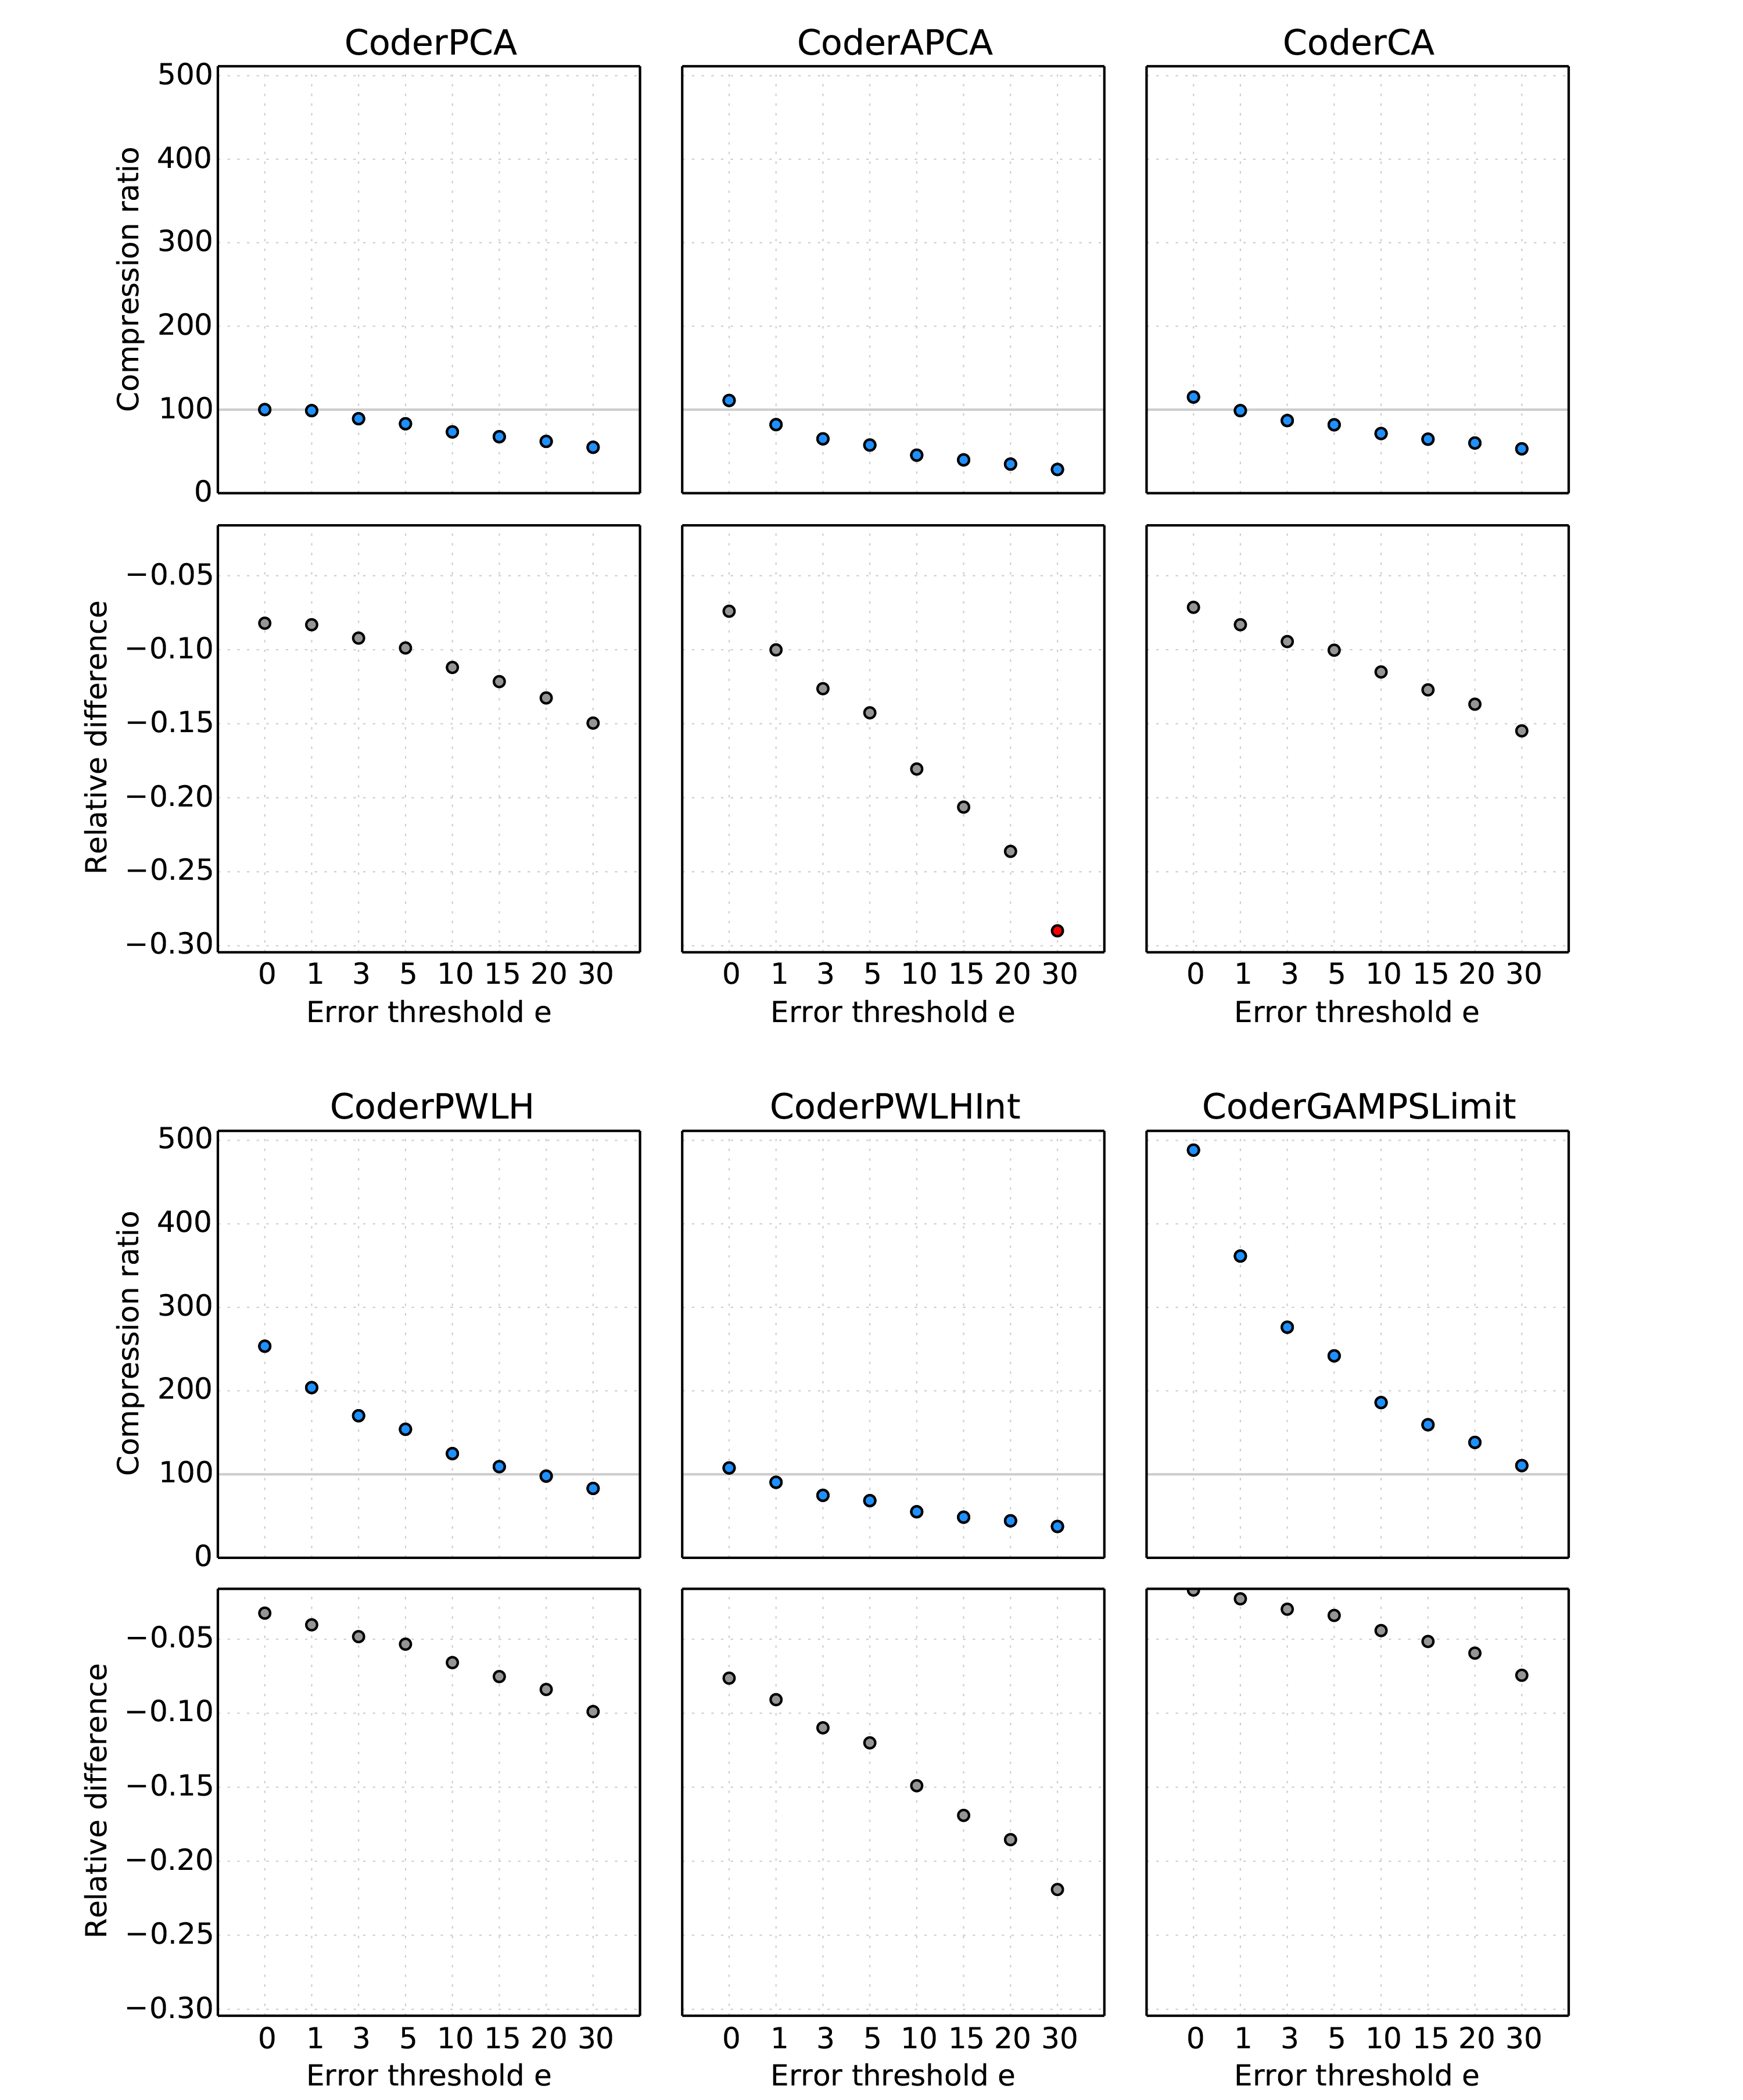
\includegraphics[scale=0.75]{chapters/Experiments/images/32-Tornado.png}
\hspace{+10pt}
\caption{\commonfigurescomp ``Longitude" data type of the \datasettornado \ dataset. In the relative difference plot for\\CoderAPCA we marked with red color the case in which \cNOmaskalgo \ obtains \\the most significant relative difference (-0.29).}
\label{fig:diff-tornado}
\end{figure}

\clearpage

\begin{figure}
\hspace{-70pt}
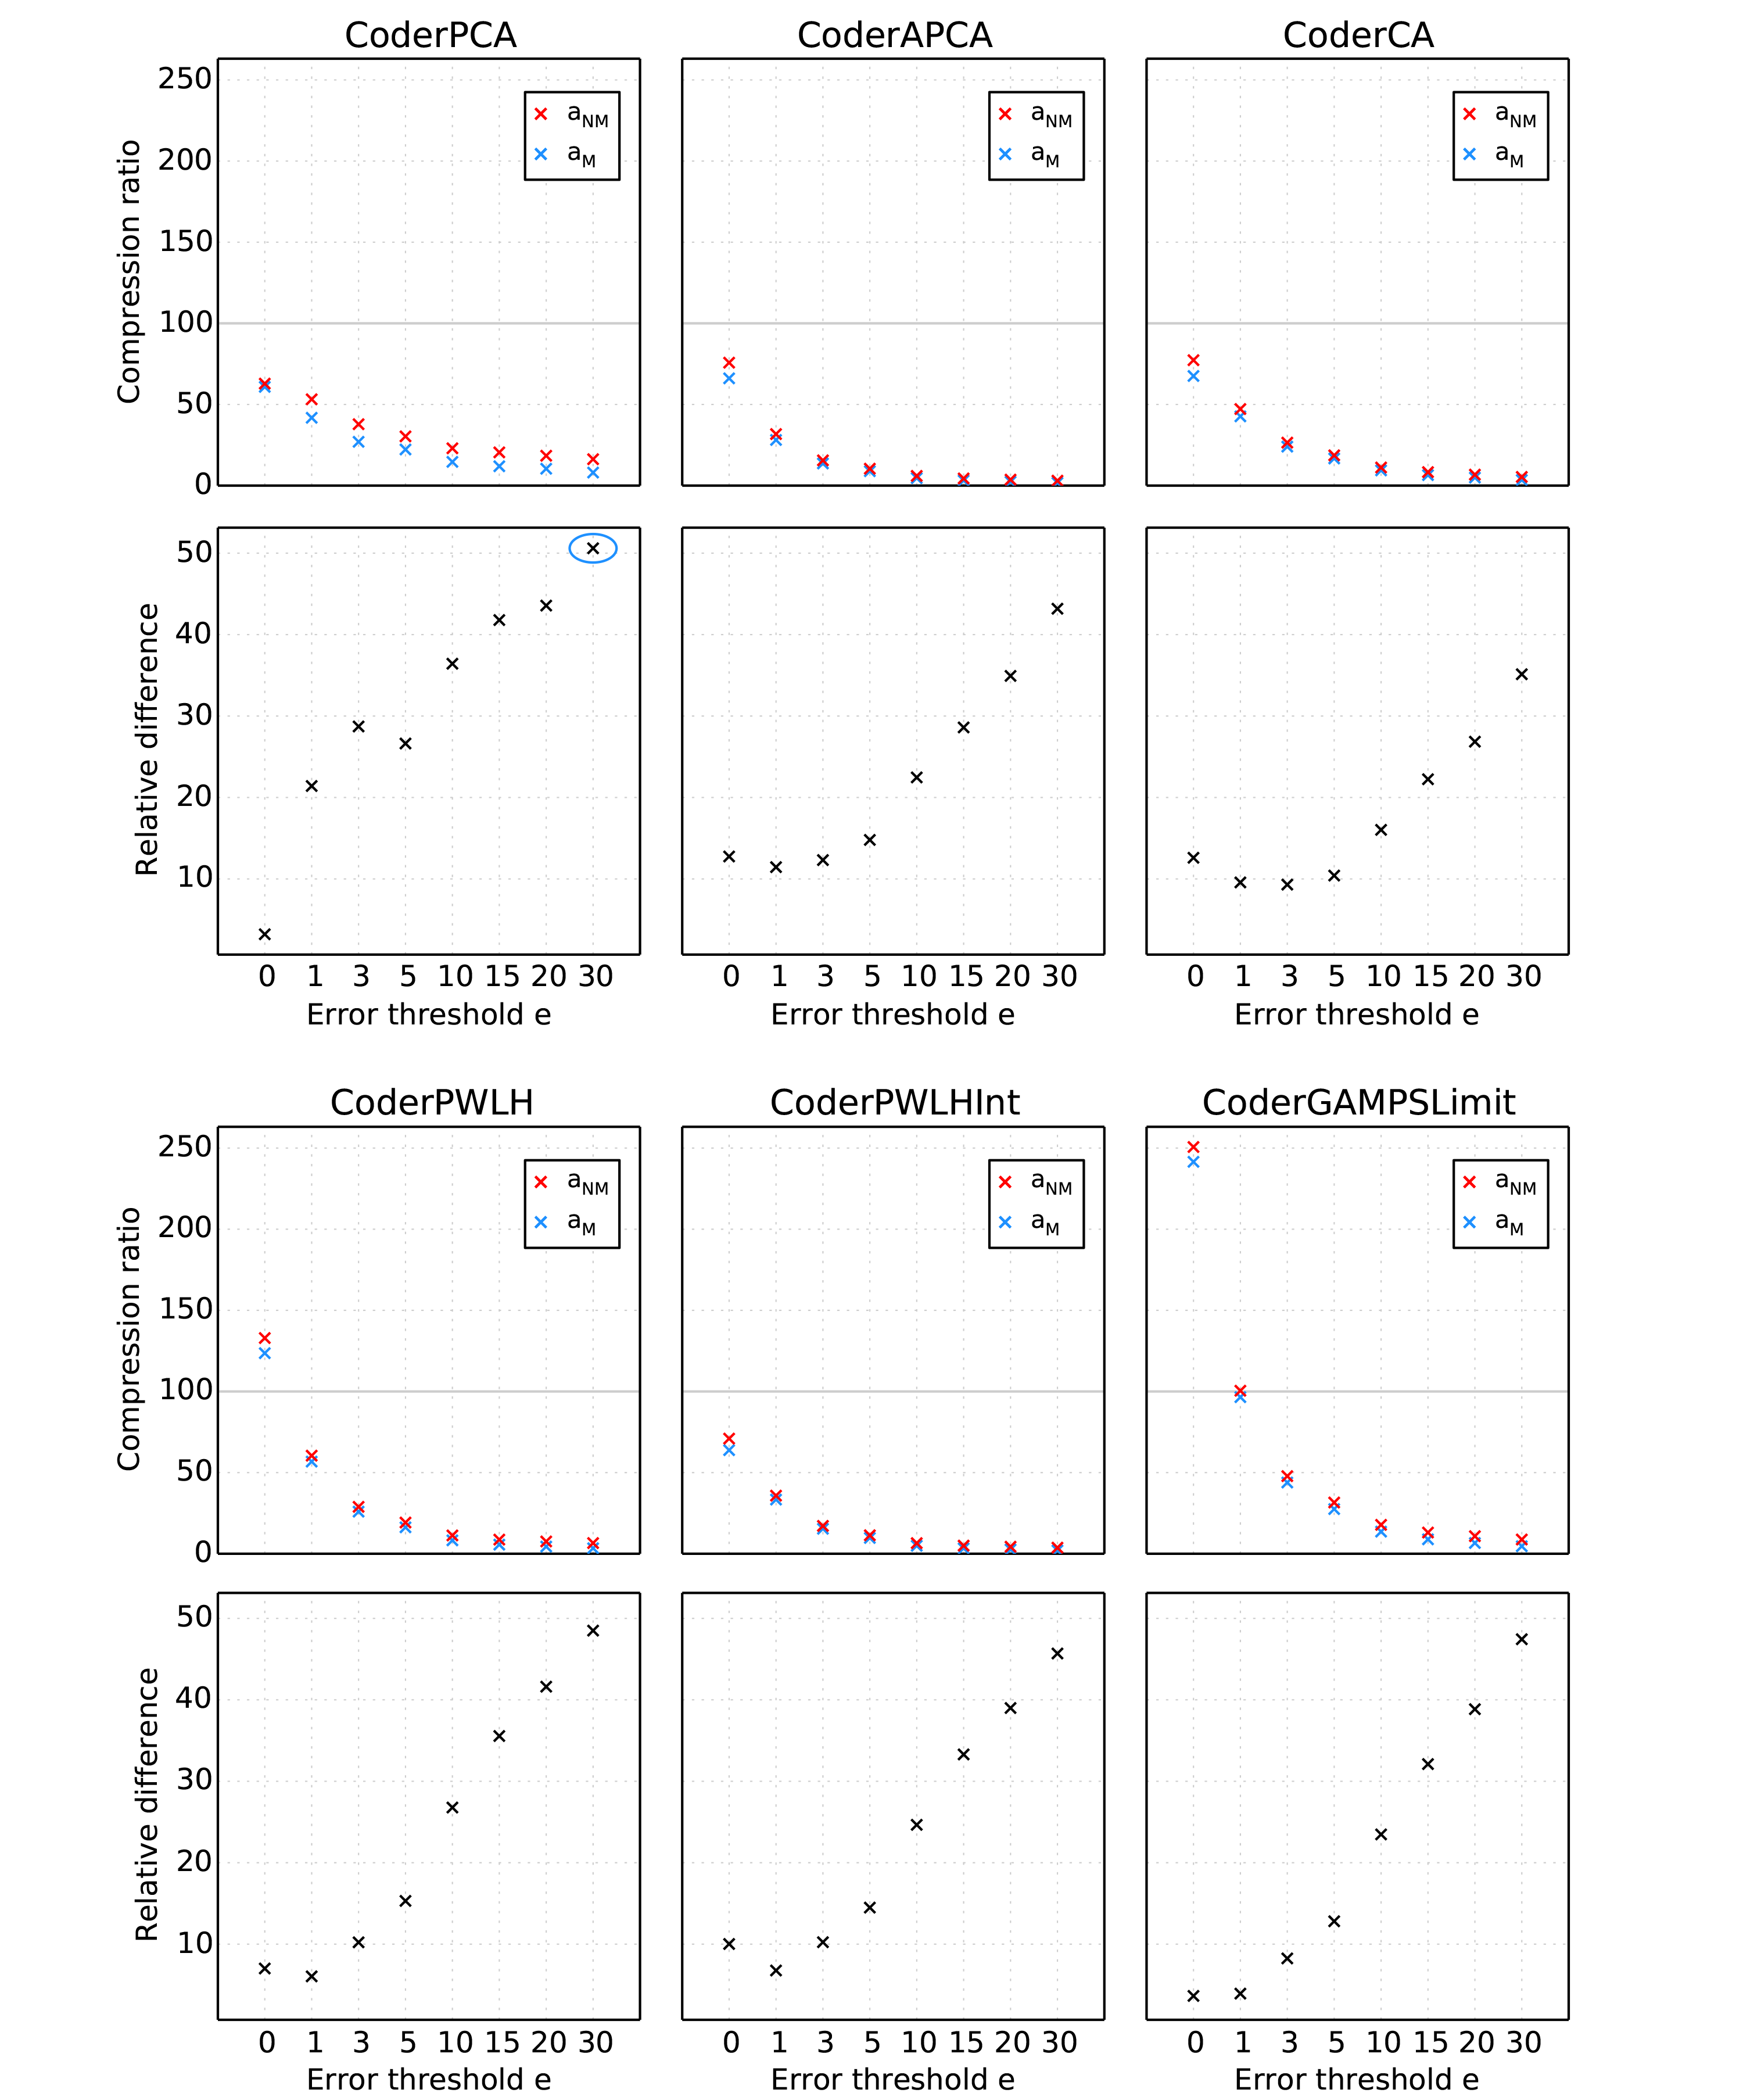
\includegraphics[scale=0.75]{chapters/Experiments/images/32-SST.png}
\hspace{+10pt}
\caption{\commonfigurescomp ``VWC" data type of the \datasetsst \ dataset. In the relative difference plot for\\CoderPCA we marked with blue color the case in which \cmaskalgo \ obtains \\the most significant relative difference (50.60).}
\label{fig:diff-sst}
\end{figure}
